\chapter{Paths, Cycles and Connectedness}

\tikzset{vtx/.style={circle,fill=black,inner sep=1.6pt}}

\section{Walks, paths and cycles}

\begin{definition}[Walk, path]
A \emph{walk} from $v_0$ to $v_k$ in $G$ is a sequence $v_0e_1v_1e_2\cdots e_kv_k$ of
vertices and edges with $e_i = v_{i-1}v_i$. Its \emph{length} is $k$ (the number of edges). A
walk is \emph{closed} if $v_0 = v_k$. A \emph{path} is a walk in which all vertices are distinct.
\end{definition}

Since our graphs have no multiple edges, a walk is determined by its vertex sequence, and we
write walks as $v_0v_1\cdots v_k$.

\begin{definition}[Cycle]
A \emph{cycle} is a subgraph isomorphic to $C_n$ for some $n \ge 3$; equivalently, a closed walk
$v_0v_1\cdots v_{k-1}v_0$ with $k\ge3$ and $v_0,\dots,v_{k-1}$ distinct. Its length is $k$. The
\emph{girth} of $G$ is the length of a shortest cycle (infinite if $G$ has no cycle).
\end{definition}

\begin{theorem}
If there is a walk from $u$ to $v$ in $G$, then there is a path from $u$ to $v$.
\end{theorem}
\begin{proof}
Take a \emph{shortest} walk $u = v_0v_1\cdots v_k = v$. If $v_i = v_j$ for some $i<j$, then
$v_0\cdots v_iv_{j+1}\cdots v_k$ is a shorter walk from $u$ to $v$, a contradiction. So the
vertices are distinct and the walk is a path.
\end{proof}

\begin{corollary}
If there is a path from $u$ to $v$ and a path from $v$ to $w$, there is a path from $u$ to $w$.
\end{corollary}
\begin{proof}
Concatenating gives a walk from $u$ to $w$.
\end{proof}

\begin{theorem}
If every vertex of $G$ has degree at least $2$, then $G$ contains a cycle.
\end{theorem}
\begin{proof}
Let $v_0v_1\cdots v_k$ be a \emph{longest} path in $G$. The vertex $v_k$ has degree at least
$2$, so it has a neighbour $w \neq v_{k-1}$. If $w$ were not on the path, $v_0\cdots v_kw$ would
be a longer path. So $w = v_i$ for some $i \le k-2$, and $v_iv_{i+1}\cdots v_kv_i$ is a cycle
(of length $k - i + 1 \ge 3$).
\end{proof}

The ``longest path'' trick is used over and over in graph theory: the end of a longest path has
all its neighbours on the path.

\section{Connectedness}

\begin{definition}[Connected]
A graph $G$ is \emph{connected} if for every two vertices $u, v$ there is a path from $u$ to $v$.
Otherwise $G$ is \emph{disconnected}: some pair of vertices is joined by no path.
\end{definition}

By the corollary above, to show $G$ is connected it suffices to fix one vertex $r$ and show
there is a path (or even a walk) from $r$ to every vertex.

\begin{example}
$K_n$ is connected (every two vertices are adjacent). The empty graph on $n \ge 2$ vertices is
disconnected.
\end{example}

\begin{example}
$Q_n$ is connected. Let $r = 00\cdots0$. From any string $s$, flip its $1$s to $0$s one at a
time; each step moves along an edge of $Q_n$, giving a walk from $s$ to $r$. Hence every vertex
is joined to $r$ and $Q_n$ is connected. (In particular $Q_{758}$ is connected.)
\end{example}

\begin{definition}[Component]
A \emph{component} of $G$ is a maximal connected subgraph. The relation ``there is a path from
$u$ to $v$'' is an equivalence relation on $V(G)$; the components are the subgraphs induced by
the equivalence classes. $G$ is connected iff it has exactly one component.
\end{definition}

\section{Cuts}

Showing that a graph is \emph{disconnected} requires a certificate too: we exhibit a set of
vertices with no edges leaving it.

\begin{definition}[Cut]
For $X \subseteq V(G)$, the \emph{cut} induced by $X$ is
$\delta(X) = \{uv \in E(G) : u \in X,\ v \notin X\}$, the set of edges with exactly one end in $X$.
\end{definition}

\begin{theorem}
$G$ is disconnected if and only if there is a non-empty proper subset $X \subsetneq V(G)$ with
$\delta(X) = \emptyset$.
\end{theorem}
\begin{proof}
($\Leftarrow$) Pick $u \in X$, $v \notin X$, and suppose $u = v_0v_1\cdots v_k = v$ is a path.
Let $i$ be the first index with $v_i \notin X$; then $i \ge 1$ and $v_{i-1}v_i \in \delta(X)$,
a contradiction. So there is no path from $u$ to $v$.

($\Rightarrow$) Suppose there is no path from $u$ to $v$. Let $X$ be the set of vertices reachable
from $u$ by a path. Then $u \in X$, $v\notin X$, and if $xy \in E(G)$ with $x \in X$, a path to $x$
followed by the edge $xy$ is a walk to $y$, so $y \in X$. Thus $\delta(X) = \emptyset$.
\end{proof}

\begin{example}
Let $V = [6]$ and $E = \{12, 23, 31, 45, 56\}$. Then $X = \{1,2,3\}$ has $\delta(X) = \emptyset$,
so the graph is disconnected; its components have vertex sets $\{1,2,3\}$ and $\{4,5,6\}$.
\end{example}

\section{Eulerian circuits}

\begin{definition}[Eulerian circuit]
An \emph{Eulerian circuit} of $G$ is a closed walk that uses every edge of $G$ exactly once.
\end{definition}

This is the K\"onigsberg bridge problem: can one walk around town crossing each bridge exactly
once and return to the start?

\begin{theorem}[Euler]
Let $G$ be a connected graph. Then $G$ has an Eulerian circuit if and only if every vertex has
even degree.
\end{theorem}
\begin{proof}
($\Rightarrow$) Each time the circuit passes through a vertex it uses two of its edges (one in,
one out); the start vertex is also left once and entered once at the end. Since each edge is used
exactly once, every degree is even.

($\Leftarrow$) Induction on $\abs{E(G)}$. If $G$ has no edges, the trivial walk works (a connected
graph with no edges has one vertex). Otherwise every vertex has even degree, and since $G$ is
connected with an edge, every vertex has degree at least $2$, so $G$ contains a cycle $C$.
Remove the edges of $C$ to get $G'$. Every vertex of $G'$ still has even degree (each lost $0$ or
$2$). Each component $H_1,\dots,H_m$ of $G'$ has fewer edges than $G$, so by induction has an
Eulerian circuit; and each $H_j$ shares a vertex with $C$ (because $G$ is connected). Now walk
around $C$, and the first time we reach a vertex of $H_j$, detour around the Eulerian circuit of
$H_j$ and return. This uses every edge of $G$ exactly once.
\end{proof}

\begin{example}
$K_5$ is $4$-regular and connected, so it has an Eulerian circuit; $K_4$ is $3$-regular, so it
does not. $Q_n$ has an Eulerian circuit iff $n$ is even.
\end{example}

\begin{aside}
Similarly, a connected graph has an Eulerian \emph{trail} (a walk using each edge once, not
necessarily closed) iff it has either $0$ or $2$ vertices of odd degree; in the latter case the
trail must start and end at the odd vertices.
\end{aside}

\section{Bridges}

\begin{definition}[Bridge]
An edge $e$ of $G$ is a \emph{bridge} if $G - e$ has more components than $G$.
\end{definition}

\begin{lemma}
If $e = uv$ is a bridge of $G$ and $H$ is the component of $G$ containing $e$, then $H - e$ has
exactly two components, one containing $u$ and the other containing $v$.
\end{lemma}
\begin{proof}
Every vertex $w$ of $H$ has a path to $u$ in $H$; if this path does not use $e$ it survives in
$H - e$, and if it does, the part before $e$ is a path from $w$ to $u$ or to $v$ that avoids $e$.
So every vertex of $H - e$ is joined to $u$ or to $v$, and there are at most two components.
Since $e$ is a bridge there are at least two, and then $u$ and $v$ must be in different ones.
\end{proof}

\begin{theorem}
An edge $e$ is a bridge if and only if $e$ is not contained in any cycle of $G$.
\end{theorem}
\begin{proof}
($\Leftarrow$, by contrapositive) Suppose $e = uv$ is in a cycle $C$. Then $C - e$ is a path from
$u$ to $v$ in $G - e$. Any walk in $G$ that uses $e$ can be rerouted along this path, so any two
vertices joined in $G$ are still joined in $G - e$, and $e$ is not a bridge.

($\Rightarrow$, by contrapositive) Suppose $e = uv$ is not a bridge. By the lemma's argument,
$u$ and $v$ lie in the same component of $G - e$, so there is a path $P$ from $u$ to $v$ in
$G - e$. Then $P$ plus $e$ is a cycle containing $e$.
\end{proof}

\begin{example}
In the graph below the edge $cd$ is a bridge (no cycle contains it); every other edge lies on one
of the two triangles.
\begin{center}
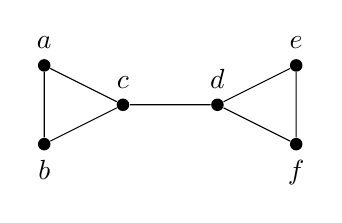
\begin{tikzpicture}
  \node[vtx,label=above:$a$] (a) at (0,1) {};
  \node[vtx,label=below:$b$] (b) at (0,-0) {};
  \node[vtx,label=above:$c$] (c) at (1,0.5) {};
  \node[vtx,label=above:$d$] (d) at (2.2,0.5) {};
  \node[vtx,label=above:$e$] (e) at (3.2,1) {};
  \node[vtx,label=below:$f$] (f) at (3.2,0) {};
  \draw (a)--(b)--(c)--(a) (c)--(d) (d)--(e)--(f)--(d);
\end{tikzpicture}
\end{center}
\end{example}

\section{Summary}
\begin{itemize}
  \item A walk from $u$ to $v$ contains a path from $u$ to $v$; minimum degree $\ge 2$ forces a cycle.
  \item Connected: a path between every pair; certify disconnectedness with a set $X$, $\emptyset\neq X\neq V$, $\delta(X)=\emptyset$.
  \item A connected graph is Eulerian iff all degrees are even.
  \item $e$ is a bridge iff it lies on no cycle; deleting a bridge splits its component in two.
\end{itemize}
